\chapter{Background}

To establish the mathematics basis and mental model of the problem, some essential conceptions in Computer Graphics are going to be introduced in this chapter.  

%%%%%%%%%%%%%%%%%%%%%%%%%%%%%%%%%%%%%%%%%%%%%%%%%%%%%%%%%%%%%%%%%%%%%%%%%%

\section{Radiometry Introduction}
Radiometry is the basic terminology to describe light which is crucial to simulation. First of all, some basic quantities have to be introduced, the related symbols are going to be defined here as well for further use.

\subsection{Important Quantities} 

\begin{table}[!ht]
\begin{center}
	\begin{tabular}{ | l | l | l |}     	
	\hline 

	Symbol & Quantity & Unit \\

	% \(Q_{\lambda}\) 	& 		Spectral radiant energy 		& 		\(J nm^{-1} \) \\
	\(Q\) 			& 		Radiant Energy 				& 		\(j\) \\ 
	\(\Phi\) 			& 		Radiant flux 					& 		\(W\) \\ 
	\(I\) 			& 		Radiant intensity 				& 		\(W sr^{-1}\) \\
	\(E\)			&		Irradiance (incident) 			&		\(W m^{-2}\) \\  
	\(L\)			&		Radiance						&		\(W m^{-2} sr^{-1}\) \\ 
	
	\hline

	\end{tabular}
\end{center} 
\caption{Radiometric symbols, names and units.}
\label{tab:radiometry_quantities}
\end{table}

\emph{Radiant energy}, \(Q\), is the energy of a collection of photons which is the basic quantity in lighting. 

\emph{Radiant flux} , \(\Phi\), is the time rate of the flow of radiant energy passing through a surface or region of space. Total emission from a light source is generally described in terms of flux. \ref{fig:flux_point_light} shows the flux emitted from a point light source measured by the total amount of energy passing through an virtual sphere around the light. 

\begin{figure}[htp] 
    \centering 
    \fbox{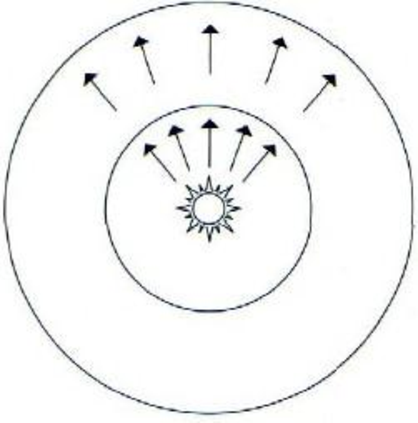
\includegraphics{flux.pdf}}
    \renewcommand{\thefigure}{\thechapter.\arabic{figure}}
    \caption[]{Radiant flux from a point light source is passing through the spheres around the light.}
    \label{fig:flux_point_light} 
\end{figure} 

\emph{Irradiance}, \(E\), is the incident (arriving at a surface location) \emph{radiant flux area density}, which is defined as the differential flux per differential area. While \emph{Radiant exitance} denoted by \(M\) is area density of flux leaving a surface.  

\begin{equation}
E(x) = \frac{d\Phi}{dA}
\end{equation}

\emph{Radiance}, \(L\), is the radiant flux per unit solid angle per unit projected area: 

\begin{equation}
L(x, \overrightarrow{\omega}) = \frac{d^{2}\Phi}{\cos{\theta} \cdot dA \cdot d\overrightarrow{\omega}}
\end{equation}

Where \(x\) is the position and \(\overrightarrow{\omega}\) is the direction. 

Radiance is the most important quantity in rendering simulation since it closely represent the color. Also radiance can be considered as the number of photons arriving per time at a small area from a given direction. Radiant energy can be computed by integrating the radiance field over all directions \(\Omega\) and area \(A\).

\begin{equation} 
\Phi = \int_{A}\int_{\Omega}L(x, \overrightarrow{\omega})(\overrightarrow{\omega} \cdot \overrightarrow{n})d\overrightarrow{\omega}dx
\label{eq:flux_from_radiance}
\end{equation} 

\begin{figure}[htp] 
    \centering 
    \fbox{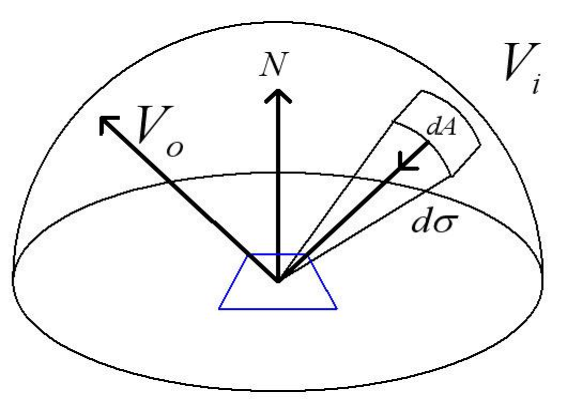
\includegraphics{solid_angle_sphere.pdf}}
    \renewcommand{\thefigure}{\thechapter.\arabic{figure}}
    \caption[]{Radiance, L, is defined as the radiant flux per unit solid angle, \(\overrightarrow{\omega}\), per unit projected area, \(dA\)}
    \label{fig:solid_angle_sphere} 
\end{figure}

The solid angle used in equation \ref{eq:flux_from_radiance} can be thought as representation of both a direction and an infinitesimal area. Therefore solid angle can also be expressed in spherical coordinates (\(\theta, \phi\))

\begin{figure}[htp] 
    \centering 
    \fbox{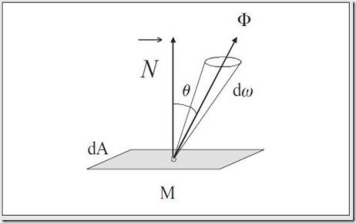
\includegraphics{radiance_solid_angle.pdf}}
    \renewcommand{\thefigure}{\thechapter.\arabic{figure}}
    \caption[]{Radiance, L, is defined as the radiant flux per unit solid angle, \(\overrightarrow{\omega}\), per unit projected area, \(dA\)}
    \label{fig:radiance_solid_angle} 
\end{figure} 

\subsection{Light Source}
The light in the form of photons is emitted from light sources. We can measure the intensity of light source in \emph{wattage}. Take a point light source for example, the power this light can emit is denoted by \(\Phi\), the emitted light distribute uniformly in all directions, the irradiance, \(E\), can be computed at a surface as: 

\begin{equation}
E(x) = \frac{\Phi \cos{\theta}}{4\pi r^{2}} 
\end{equation}

Where \(r\) is the distance from \(x\) to the light source and \(\theta\) is the angle between the surface normal and the direction to the light source. From the equation we can intuitively tell a surface facing the source will receive more photons per area than a surface that is oriented differently.   

%%%%%%%%%%%%%%%%%%%%%%%%%%%%%%%%%%%%%%%%%%%%%%%%%%%%%%%%%%%%%%%%%%%%%%%%%%


\section{Render Equation}
With the physically-based model of lighting, a theoretical framework describing the interaction between light and an surface will be introduced in this section. 

\begin{figure}[htp] 
    \centering 
    \fbox{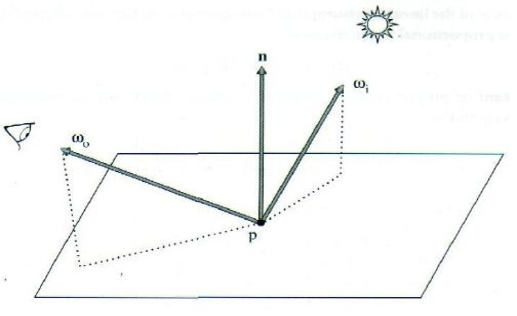
\includegraphics{brdf.pdf}}
    \renewcommand{\thefigure}{\thechapter.\arabic{figure}}
    \caption[]{The geometric setup of BRDF. }
    \label{fig:brdf} 
\end{figure} 

The \emph{Bidirectional Reflectance Distribution Function}, BRDF, is the mathematic tool describing the reflectiona of light encounters an surface. To define the BRDF, the geometric configuration is shown in figure \ref{fig:brdf}. \(\omega_{i}\) is the incident lighting direction, \(\omega_{o}\) is the direction in which the reflected light leaving from the surface, \(n\) is the normal vector at the location \(p\) on the surface. Given the incident radiance \(L_{i}(p, \omega_{i})\), we are finding out the outgoing radiance to the viewer, \(L_{o}(p, \omega_{o})\). 

The BRDF, \(f_{r}\), defines the relationship between differential reflected radiance and differential irradiance: 

\begin{equation}
f_{r} = \frac{dL_{o}(p, \omega_{o})}{dE(p, \omega_{i})} = \frac{dL_{o}(p, \omega_{o})}{L_{i}(p, \omega_{i})(\omega_{i} \cdot n)d\omega{i}}
\label{eq:brdf}
\end{equation} 

There are two important properties of BRDF used in rendering. The first one is the Helmholtz's law of reciprocity, that is given any pair of directions \( (\omega_{i}, \omega_{o} ) \), we have: 

\begin{equation}
f_{r}(p, \omega_{i}, \omega_{o}) = f_r(p, \omega_{o}, \omega_{i})
\end{equation}

Another important physical property of BRDF is energy conservation, stating that the total reflected energy is less than or equal to the incident energy. For all direction \( \omega_{o} \).

\begin{equation}
 \int_{\Omega}f_{r}(p, \omega_{i}, \omega_{o})L_{i}(p, \omega_{i})(\omega_{i} \cdot n)d\omega_{i} \leq 1 , \forall \omega_{i}
\end{equation}

Given the definition of BRDF, we can introduce the basic render equation, also known as \emph{local illumination model} by integrating the equation \ref{eq:brdf} over the sphere of incident directions around location \(p\), the left side of the equation will be the outgoding radiance in direction \(\omega_{o}\).

\begin{equation}
L_{o}(p, \omega_{o}) = \int_{\Omega}f_{r}(p, \omega_{i}, \omega_{o})L_{i}(p, \omega_{i})(\omega_{i} \cdot n)d\omega_{i}
\label{eq:local_render_equation}
\end{equation}

Where \(\Omega\) is the hemisphere of incoming directions at \(p\).

\paragraph{Light Transport Equationa} 

The local illumiation model is used to describe the direct lighting effect which is too simple for simulating real-world lighting effect, indirect lighting has to be introduced to this model as well. Therefore we introduce the Light Transport Equation (LTE) in this section to form the mathematical basis for all global illumination algorithms, The LTE states the necessary conditions for equilibrium of light transport in the scene without participating media. 

\begin{equation}
L_{o}(p, \omega_{o}) = L_{e}(p, \omega_{o}) + \int_{\Omega}f_{r}(p, \omega_{i}, \omega_{o})L_{i}(p, \omega_{i})(\omega_{i} \cdot n)d\omega_{i}
\label{eq:lte}
\end{equation}

%%%%%%%%%%%%%%%%%%%%%%%%%%%%%%%%%%%%%%%%%%%%%%%%%%%%%%%%%%%%%%%%%%%%%%%%%%

\section{Monte-Carlo Ray Tracing} 


